{
I bilag \ref{app_source1} er kildekoden til vores \textbf{R}-program inkluderet.
Funktionen \texttt{assignment1()} løser den første opgave. Vi bruger et
\emph{for-loop} til at gå gennem en vektor, hvori vi har defineret de tre
antalsparametre. Koden er i øvrigt flot indenteret og selvdokumenterende.

Centralt i funtionen \texttt{assignment1()} har vi metoden fra
\textbf{R} kaldet \texttt{dbinom(x, n, p)}. Denne metode er defineret som
binomialfordelingens sandsynlighedsfunktion som er givet ved

\begin{equation}
    p(x) = \binom{n}{x}p^{x}(1 - p)^{n - x}
    \label{binomsshf}
\end{equation}

Hvis $x$ er en vektor vil \textbf{R} returnere en vektor med resultatet
fra ligning \ref{binomsshf}. Vi kan da plotte resultatet med metoden
\texttt{plot()} i \textbf{R}.

I programmets løkke sættes for hver iteration et nyt filnavn til plottet.
Vi eksporterer plottet til et png-billede. I figur \ref{binom8_20_100}
ses resultatet fra programmet.

\begin{figure}[!h]
    \centering
    \subfloat[$n = 8$ og $p = 0.25$]{
        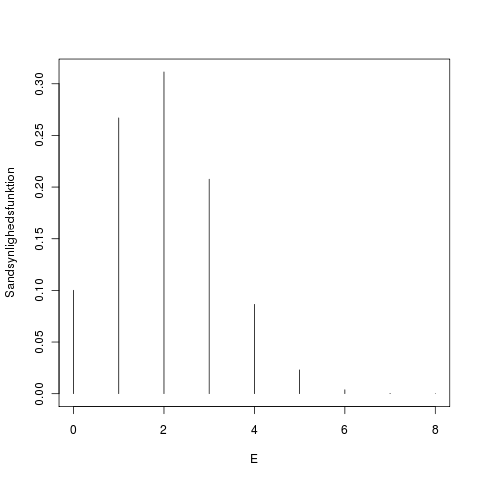
\includegraphics[width=0.5\textwidth]{8_plot_1}
        \label{binom_8}
    }
    \subfloat[$n = 20$ og $p = 0.25$]
        {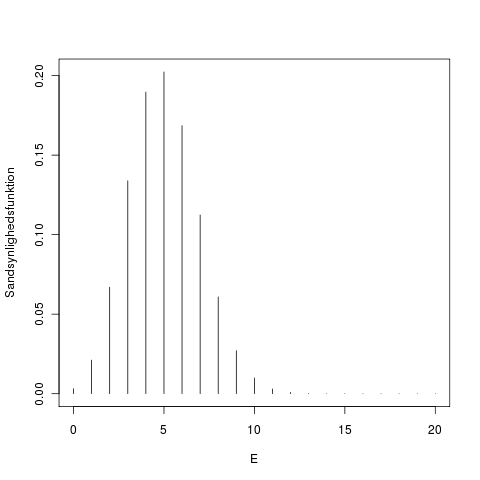
\includegraphics[width=0.5\textwidth]{20_plot_1}
        \label{binom_20}
    }\\
    \subfloat[$n = 100$ og $p = 0.25$]{
        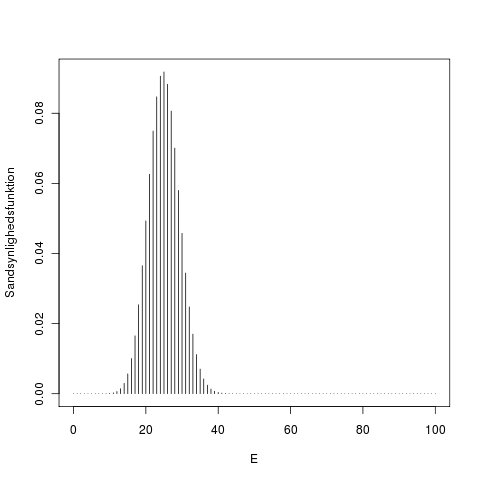
\includegraphics[width=0.5\textwidth]{100_plot_1}
        \label{binom_100}
    }
    \caption{Resultater fra binomialfordelinger med antalsparameter 8, 20
    og 100 og sandsynlighedsparameter $\frac{1}{4}$}
    \label{binom8_20_100}
\end{figure}

}
